\documentclass[a5paper, 10pt]{article}

% Текст
\usepackage[utf8]{inputenc} % UTF-8 кодировка
\usepackage[russian]{babel} % Русский язык
\usepackage{indentfirst} % красная строка в первом параграфе в главе
% Отображение страниц
\usepackage{geometry} % размеры листа и отступов
\geometry{
	left=12mm,
	top=25mm,
	right=15mm,
	bottom=17mm,
	marginparsep=0mm,
	marginparwidth=0mm,
	headheight=10mm,
	headsep=7mm,
	nofoot}
\usepackage{afterpage,fancyhdr} % настройка колонтитулов
\pagestyle{fancy}
\fancypagestyle{style}{ % создание нового стиля style
	\fancyhf{} % очистка колонтитулов
	\fancyhead[LO, RE]{} % название документа наверху
	\fancyhead[RO, LE]{\leftmark} % название section наверху
	\fancyfoot[RO, LE]{\thepage} % номер страницы справа внизу на нечетных и слева внизу на четных
	\renewcommand{\headrulewidth}{0.25pt} % толщина линии сверху
	\renewcommand{\footrulewidth}{0pt} % толцина линии снизу
}
\fancypagestyle{plain}{ % создание нового стиля plain -- полностью пустого
	\fancyhf{}
	\renewcommand{\headrulewidth}{0pt}
}
\fancypagestyle{title}{ % создание нового стиля title -- для титульной страницы
	\fancyhf{}
	\fancyhead[C]{{\footnotesize
			Министерство образования и науки Российской Федерации\\
			Федеральное государственное автономное образовательное учреждение высшего образования
	}}
	\fancyfoot[C]{{\large 
			Санкт-Петербург, 2023
	}}
	\renewcommand{\headrulewidth}{0pt}
}

% Математика
\usepackage{amsmath, amsfonts, amssymb, amsthm} % Набор пакетов для математических текстов
%\usepackage{dmvnbase} % мехматовский пакет latex-сокращений
\usepackage{cancel} % зачеркивание для сокращений
% Рисунки и фигуры
\usepackage[pdftex]{graphicx} % вставка рисунков
\usepackage{wrapfig, subcaption} % вставка фигур, обтекая текст
\usepackage{caption} % для настройки подписей
\captionsetup{figurewithin=none,labelsep=period, font={small,it}} % настройка подписей к рисункам
% Рисование
\usepackage{tikz} % рисование
\usepackage{circuitikz}
\usepackage{pgfplots} % графики
% Таблицы
\usepackage{multirow} % объединение строк
\usepackage{multicol} % объединение столбцов
% Остальное
\usepackage[unicode, pdftex]{hyperref} % гиперссылки
\usepackage{enumitem} % нормальное оформление списков
\setlist{itemsep=0.15cm,topsep=0.15cm,parsep=1pt} % настройки списков
% Теоремы, леммы, определения...
\theoremstyle{definition}
\newtheorem{Def}{Определение}
\newtheorem*{Axiom}{Аксиома}
\theoremstyle{plain}
\newtheorem{Th}{Теорема}
\newtheorem{Lem}{Лемма}
\newtheorem{Cor}{Следствие}
\newtheorem{Ex}{Пример}
\theoremstyle{remark}
\newtheorem*{Note}{Замечание}
\newtheorem*{Solution}{Решение}
\newtheorem*{Proof}{Доказательство}
% Свои команды
\newcommand{\comb}[1]{\left[\hspace{-4pt}\begin{array}{l}#1\end{array}\right.\hspace{-5pt} } % совокупность уравнений
% Титульный лист
\usepackage{csvsimple-l3}
\newcommand*{\titlePage}{
	\thispagestyle{title}
	\begingroup
	\begin{center}
		%		{\footnotesize
			%			Министерство образования и науки Российской Федерации\\
			%			Федеральное государственное автономное образовательное учреждение высшего образования
			%		}
		%		
		\vspace*{6ex}
		
		{\small
			САНКТ-ПЕТЕРБУРГСКИЙ НАЦИОНАЛЬНЫЙ ИССЛЕДОВАТЕЛЬСКИЙ УНИВЕРСИТЕТ ИНФОРМАЦИОННЫХ ТЕХНОЛОГИЙ, МЕХАНИКИ И ОПТИКИ	
		}
		
		\vspace*{2ex}
		
		{\normalsize
			Факультет систем управления и робототехники
		}
		
		\vspace*{15ex}
		
		{\Large \bfseries 
			Лабораторная работа № 2\\
"Тригонометрические ряды Фурье"
		}
\vspace*{2ex}
		
		{\normalsize
			по дисциплине "Математический анализ"
		}

                    \vspace*{2ex}

                    { \bfseries 
			Вариант № 20
		}
	\end{center}
	\vspace*{20ex}
	\begin{flushright}
		{\large 
			\underline{Выполнила}: студентка гр. \textbf{R3138}\\
			\begin{flushright}
				\textbf{Нечаева А. А.}\\
			\end{flushright}
		}
		
		\vspace*{5ex}
		
		{\large 
			\underline{Преподаватель}: \textit{Бойцев А. А.}
		}
	\end{flushright}	
	\newpage
	\setcounter{page}{2}
	\endgroup}

\begin{document}
	\titlePage
	\pagestyle{style}
\newpage

\section{Аналитическая часть}
Заданная функция:
\begin{equation}
f(x) = 
\begin{cases}
0, \, & x \in [0, \, 1);\\
2 - x, \, & x \in [1, 2].
\end{cases}
\end{equation}


\subsection{Построение общего тригонометрического ряда}	
$f(x)$ определена на $[0, 2]$. Преобразуем:
\begin{equation*}
0 \leq x \leq 2  \, \, \to \, \,
0 \leq \pi x \leq 2 \pi \, \, \to \, \,
-\pi \leq \pi(x-1) \leq \pi\\
\end{equation*}
Новая переменная $t =\pi(x-1)$. Выразим $x = \frac{t}{\pi} + 1$ и запишем новую функцию $\phi (t) = f( \frac{t}{\pi} + 1)$. $\phi (t)$ определена на отрезке $[-\pi, \, \pi]$ .\\
Функция $\phi (t)$ удовлетворяет условию теоремы Дирихле о разложении периодической функции в ряд Фурье.
\begin{equation*}
\phi (t) \sim  \frac{a_0}{2} + \sum \limits_{n = 1}^{\infty} \left( a_n \cos(nt) + b_n \sin(nt) \right), 
\end{equation*}
где $a_0, \, a_n, \, b_n$ -- коэффициенты Фурье:\\
\begin{equation*}
a_0 = \frac{1}{\pi} \int \limits_{-\pi}^{\pi} \phi(t) \, dt,
\end{equation*}
\begin{equation*}
a_n = \frac{1}{\pi} \int \limits_{-\pi}^{\pi} \phi(t) \cos(nt) \, dt,
\end{equation*}
\begin{equation*}
b_n = \frac{1}{\pi} \int \limits_{-\pi}^{\pi} \phi(t) \sin(nt) \, dt.
\end{equation*}
Проведем обратную замену $t =\pi(x-1)$:
\begin{equation*}
f (x) \sim  \frac{a_0}{2} + \sum \limits_{n = 1}^{\infty} \left( a_n \cos(\pi n(x-1)) + b_n \sin(\pi n(x-1)) \right),
\end{equation*}
\begin{equation*}
a_0 = \frac{1}{\pi} \int \limits_{0}^{2} f(x) \pi \, dx = \int \limits_{0}^{2} f(x) \, dx, 
\end{equation*}
\begin{equation*}
a_n = \frac{1}{\pi} \int \limits_{0}^{2} f(x) \cos(\pi n(x-1))  \pi \, dx = \int \limits_{0}^{2} f(x) \cos(\pi n(x-1)) \, dx ,
\end{equation*}
\begin{equation*}
b_n = \frac{1}{\pi} \int \limits_{0}^{2} f(x) \sin(\pi n(x-1)) \pi \, dx = \int \limits_{0}^{2} f(x) \sin(\pi n(x-1)) \, dx .
\end{equation*}

Вычислим значения коэффициетов:
\begin{equation*}
a_0 = \int \limits_{0}^{2} f(x) \, dx = \int \limits_{0}^{1} 0 \, dx + \int \limits_{1}^{2} 2 - x \, dx = \frac{1}{2}
\end{equation*}
\begin{multline*}
a_n  = \int \limits_{0}^{2} f(x) \cos(\pi n(x-1)) \, dx = \int \limits_{1}^{2} (2-x) \cos(\pi n(x-1)) \, dx \, \, \fbox{=}
\end{multline*}
Вычислим неопределенный интеграл:
\begin{multline*}
 \int  (2-x) \cos(\pi n(x-1)) \, dx = 
\begin{Vmatrix}
v = 2-x \, & dv = -dx\\
du = \cos(\pi n(x-1)) \, dx \, & u = \frac{\sin(\pi n(x-1))}{\pi n}
\end{Vmatrix}
= \\ =  \frac{(2-x) \sin(\pi n(x-1))}{\pi n} + \frac{1}{\pi n} \int \sin(\pi n(x-1)) \, dx = \\=
 \frac{(2-x) \sin(\pi n(x-1))}{\pi n} -  \frac{\cos (\pi n(x-1))}{(\pi n)^2} + C
\end{multline*}

\begin{equation*}
\fbox{=} -  \frac{\cos (\pi n)}{(\pi n)^2} + \frac{\cos (0)}{(\pi n)^2} = \frac{1}{(\pi n)^2} -  \frac{(-1)^n}{(\pi n)^2}
\end{equation*}
\begin{equation*}
b_n  = \int \limits_{0}^{2} f(x) \sin(\pi n(x-1)) \, dx  =  \int \limits_{1}^{2} (2-x) \sin(\pi n(x-1)) \, dx \, \, \fbox{=}
\end{equation*}
Вычислим неопределенный интеграл:
\begin{multline*}
 \int  (2-x) \sin(\pi n(x-1)) \, dx = 
\begin{Vmatrix}
v = 2-x \, & dv = -dx\\
du = \sin(\pi n(x-1)) \, dx \, & u = -\frac{\cos(\pi n(x-1))}{\pi n}
\end{Vmatrix}
= \\ =  - \frac{(2-x) \cos(\pi n(x-1))}{\pi n} - \frac{1}{\pi n} \int \cos(\pi n(x-1)) \, dx = \\=
 -\frac{(2-x) \cos(\pi n(x-1))}{\pi n} -  \frac{\sin (\pi n(x-1))}{(\pi n)^2} + C
\end{multline*}
\begin{equation*}
\fbox{=} \frac{1}{\pi n}
\end{equation*}
Запишем итоговую формулу для разложения в тригонометрический ряд Фурье:
\begin{equation*}
f (x) \sim  \frac{1}{4} + \sum \limits_{n = 1}^{\infty} \left( \left( \frac{1}{(\pi n)^2} -  \frac{(-1)^n}{(\pi n)^2}  \right) \cos(\pi n(x-1)) +  \left( \frac{1}{\pi n} \right) \sin(\pi n(x-1)) \right)
\end{equation*}


\newpage
\subsection{Построение ряда Фурье по синусам}
Доопределим функцию $f(x)$ на отрезке $[-2, 0]$ четным образом, то есть $f(x) = -f(-x), \, x \in [-2, 0]$. Для полученной четной функции на отрезке $[-2, 2]$ строим ряд Фурье:
\begin{equation*} 
f(x) \sim  \sum \limits_{n=1}^{\infty} b_n \sin \frac{\pi n x}{2},
\end{equation*}
где
\begin{equation*} 
b_n =  \int \limits_{0}^{2} f(x) \sin \frac{\pi n x}{2} \, dx
\end{equation*}
Рассматриваем сумму этого ряда только на отрезке $[0, 2]$ и получаем разложение исходной функции $f(x)$ на отрезке  $[0, 2]$ в ряд Фурье по синусам.\\
Вычислим значение коэффициента:
\begin{equation*} 
b_n =  \int \limits_{1}^{2} (2-x) \sin \frac{\pi n x}{2} \, dx \, \, \fbox{=}
\end{equation*}
Вычислим неопределенный интеграл:
\begin{multline*} 
 \int  (2-x) \sin \frac{\pi n x}{2} \, dx = 
\begin{Vmatrix}
v = 2-x \, & dv = -dx\\
du =   \sin \frac{\pi n x}{2} \, dx \, & u = -\frac{2 \cos \left( \frac{\pi n x}{2}\right)}{\pi n}
\end{Vmatrix}
=\\= - \frac{2 (2-x) \cos \left( \frac{\pi n x}{2}\right)}{\pi n} - \int \frac{2 \cos \left( \frac{\pi n x}{2}\right)}{\pi n}  \, dx =
-\frac{2 (2-x) \cos \left( \frac{\pi n x}{2}\right)}{\pi n} - \frac{4 \sin \left( \frac{\pi n x}{2} \right)}{(\pi n)^2} + C
\end{multline*}
\begin{equation*} 
 \fbox{=} \frac{4 \sin \left( \frac{\pi n}{2}\right)}{(\pi n)^2} + \frac{2 \cos \left( \frac{\pi n}{2}\right)}{\pi n}
\end{equation*}
Запишем итоговое разложение функции в ряд Фурье по синусам:
\begin{equation*} 
f(x) \sim  \sum \limits_{n=1}^{\infty} \left( \frac{4 \sin \left( \frac{\pi n}{2}\right)}{(\pi n)^2} + \frac{2 \cos \left( \frac{\pi n}{2}\right)}{\pi n} \right) \sin \frac{\pi n x}{2}
\end{equation*}


\newpage
\subsection{Построение ряда Фурье по косинусам}
Непериодическая функция $f(x)$ задана на отрезке $[0, 2]$. Доопределим функцию $f(x)$ на отрезке $[-2, 0]$ четным образом, то есть $f(x) = f(-x), \, x \in [-2, 0]$. Для полученной четной функции на отрезке $[-2, 2]$ строим ряд Фурье:
\begin{equation*} 
f(x) \sim  \frac{a_0}{2} + \sum \limits_{n=1}^{\infty} a_n \cos \frac{\pi n x}{2},
\end{equation*}
где
\begin{equation*} 
a_0 = \frac{2}{2} \int \limits_{0}^{2} f(x) \, dx = \int \limits_{0}^{2} f(x) \, dx
\end{equation*}
\begin{equation*} 
a_n =  \int \limits_{0}^{2} f(x) \cos \frac{\pi n x}{2} \, dx
\end{equation*}
Рассматриваем сумму этого ряда только на отрезке $[0, 2]$ и получаем разложение исходной функции $f(x)$ на отрезке  $[0, 2]$ в ряд Фурье по косинусам.\\
Вычислим значения коэффициентов:
\begin{equation*} 
a_0 = \int \limits_{0}^{2} f(x) \, dx =  \int \limits_{1}^{2} (2-x) \, dx = \frac{1}{2}
\end{equation*}
\begin{equation*} 
a_n =  \int \limits_{0}^{2} f(x) \cos \frac{\pi n x}{2} \, dx = \int \limits_{1}^{2} (2-x) \cos \frac{\pi n x}{2} \, dx \, \, \fbox{=}
\end{equation*}
Вычислим неопределенный интеграл:
\begin{multline*} 
 \int  (2-x) \cos \frac{\pi n x}{2} \, dx = 
\begin{Vmatrix}
v = 2-x \, & dv = -dx\\
du =   \cos \frac{\pi n x}{2} \, dx \, & u = \frac{2 \sin \left( \frac{\pi n x}{2}\right)}{\pi n}
\end{Vmatrix}
=\\= \frac{2 (2-x) \sin \left( \frac{\pi n x}{2}\right)}{\pi n} + \int \frac{2 \sin \left( \frac{\pi n x}{2}\right)}{\pi n}  \, dx =
\frac{2 (2-x) \sin \left( \frac{\pi n x}{2}\right)}{\pi n} - \frac{4 \cos \left( \frac{\pi n x}{2} \right)}{(\pi n)^2} + C
\end{multline*}

\begin{equation*} 
\fbox{=} - \frac{4 \cos \left( \pi n x \right)}{(\pi n)^2} - \frac{2 \sin \left( \frac{\pi n}{2}\right)}{\pi n} + \frac{4 \cos \left( \frac{\pi n }{2} \right)}{(\pi n)^2} = - \frac{4 \left( -1 \right)^n}{(\pi n)^2} - \frac{2 \sin \left( \frac{\pi n}{2}\right)}{\pi n} + \frac{4 \cos \left( \frac{\pi n }{2} \right)}{(\pi n)^2} 
\end{equation*}
Запишем итоговое разложение функции в ряд Фурье по косинусам:
\begin{equation*} 
f(x) \sim  \frac{1}{4} + \sum \limits_{n=1}^{\infty} \left(- \frac{4 \left( -1 \right)^n}{(\pi n)^2} - \frac{2 \sin \left( \frac{\pi n}{2}\right)}{\pi n} + \frac{4 \cos \left( \frac{\pi n }{2} \right)}{(\pi n)^2} \right) \cos \frac{\pi n x}{2}
\end{equation*}


\newpage

\section{Работа программы}
Программа написана на языке \textit{Python 3.9} с тспользованием библиотеки \textit{Manim}.

\begin{figure}[h!]
		\begin{center}
			\begin{subfigure}{0.7\linewidth}
				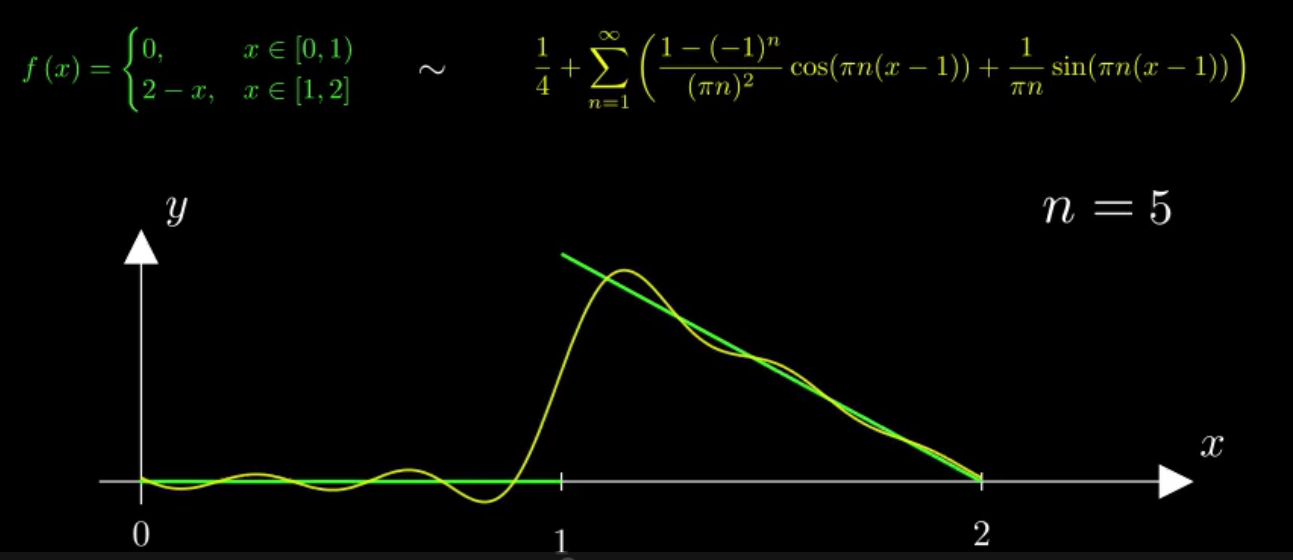
\includegraphics[width=\linewidth]{"./pictures/o_5.png"}
				\caption{при $n=5$}
			\end{subfigure}
			\begin{subfigure}{0.7\linewidth}
				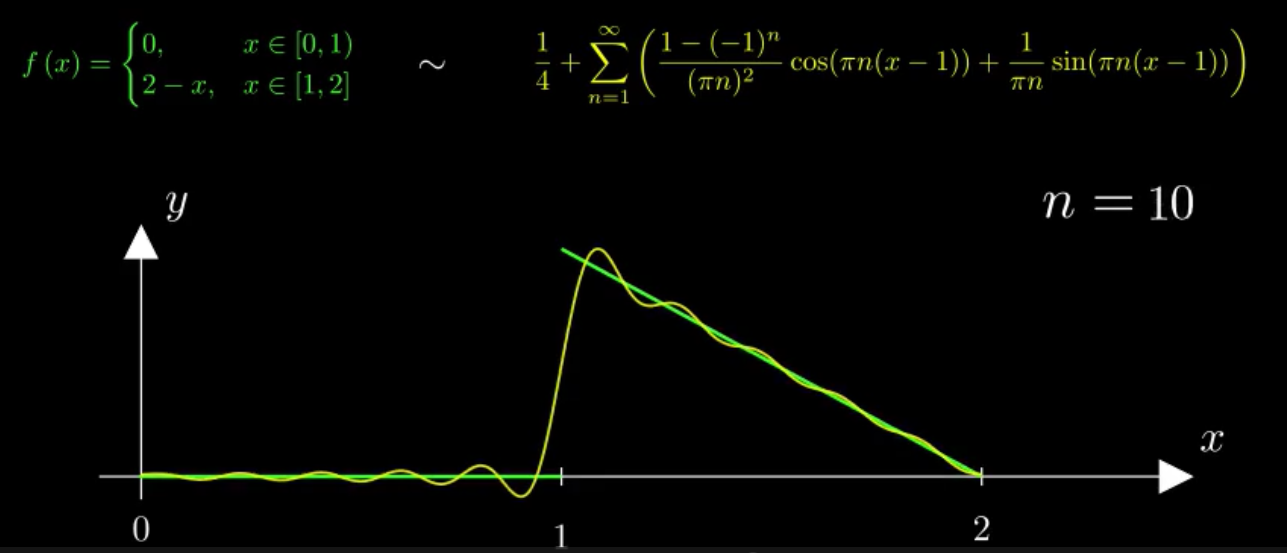
\includegraphics[width=\linewidth]{"./pictures/o_10.png"}
				\caption{при $n=10$}
			\end{subfigure}
			\begin{subfigure}{0.7\linewidth}
				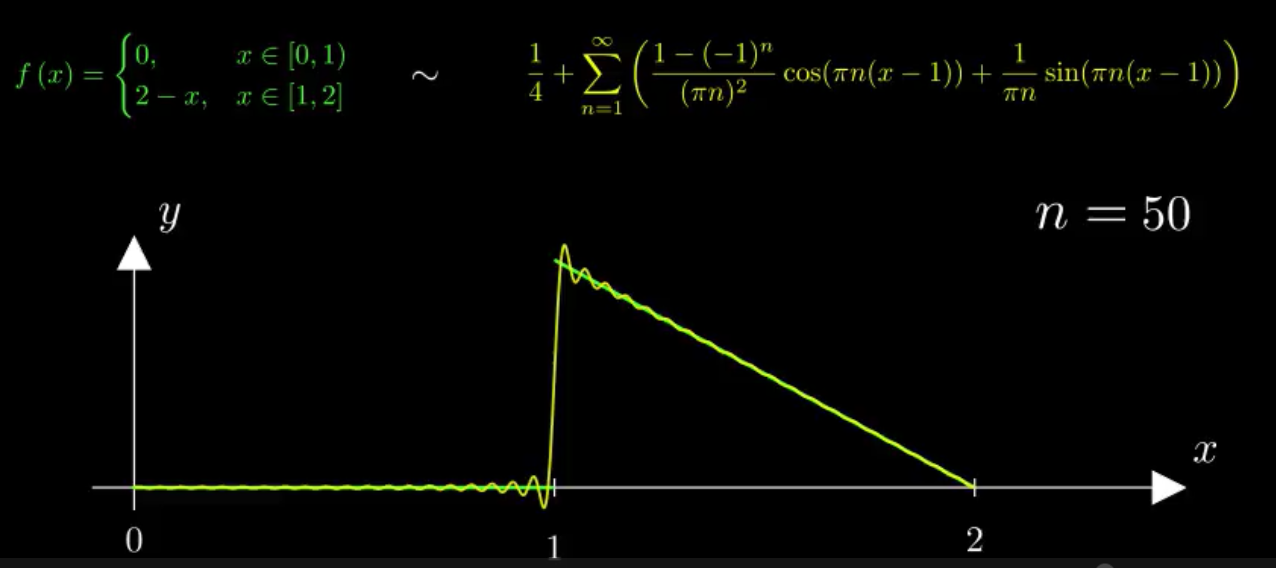
\includegraphics[width=\linewidth]{"./pictures/o_50.png"}
				\caption{при $n=50$}
			\end{subfigure}
		\caption{Результаты работы программы при различных $n$ для общего тригонометрического ряда Фурье}\label{result}
		\end{center}
	\end{figure}

\begin{figure}
		\begin{center}
			\begin{subfigure}{0.7\linewidth}
				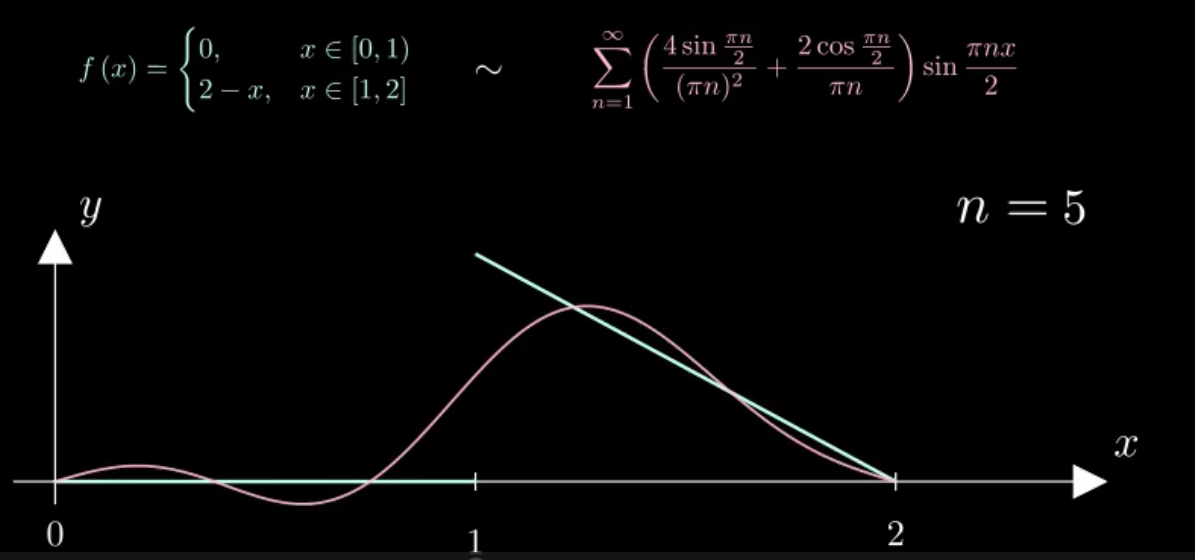
\includegraphics[width=\linewidth]{"./pictures/s_5.png"}
				\caption{при $n=5$}
			\end{subfigure}
			\begin{subfigure}{0.7\linewidth}
				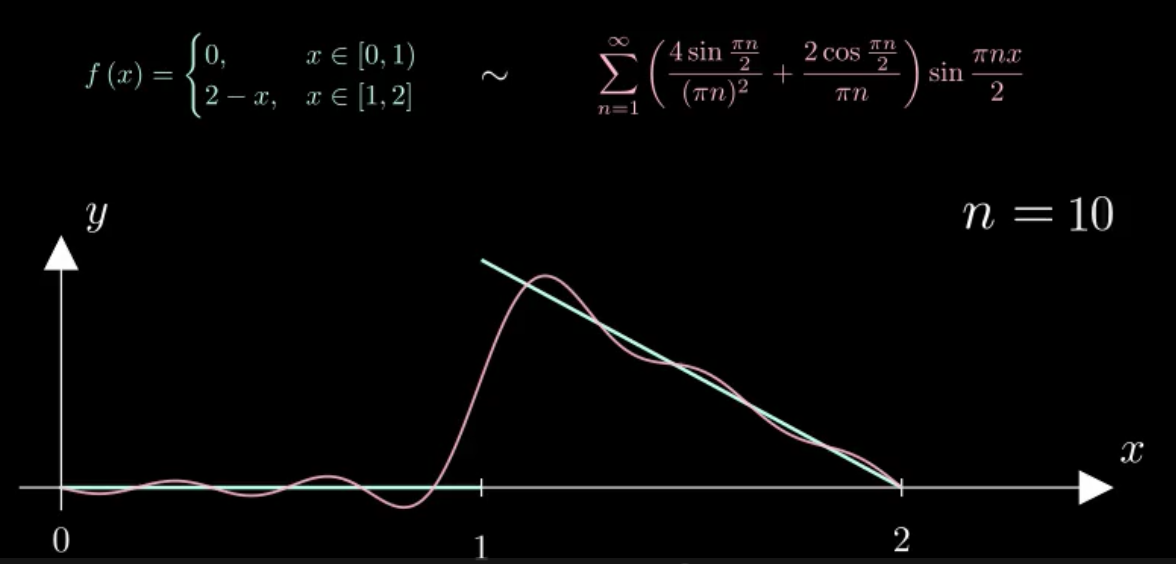
\includegraphics[width=\linewidth]{"./pictures/s_10.png"}
				\caption{при $n=10$}
			\end{subfigure}
			\begin{subfigure}{0.7\linewidth}
				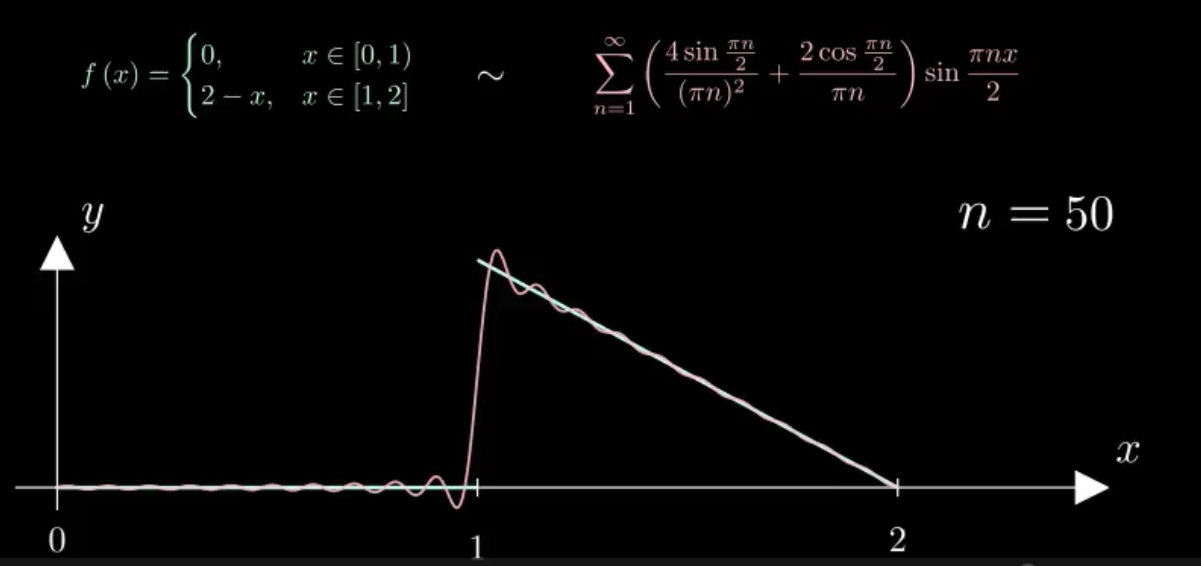
\includegraphics[width=\linewidth]{"./pictures/s_50.png"}
				\caption{при $n=50$}
			\end{subfigure}
		\caption{Результаты работы программы при различных $n$ для разложения в ряд Фурье по синусам}\label{result}
		\end{center}
	\end{figure}

\begin{figure}
		\begin{center}
			\begin{subfigure}{0.7\linewidth}
				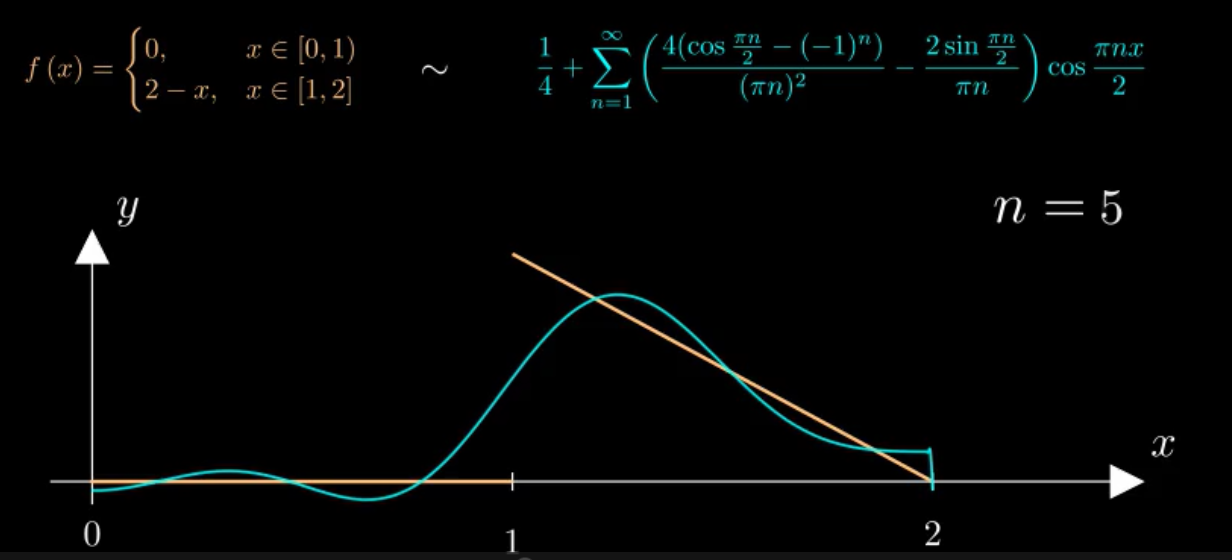
\includegraphics[width=\linewidth]{"./pictures/c_5.png"}
				\caption{при $n=5$}
			\end{subfigure}
			\begin{subfigure}{0.7\linewidth}
				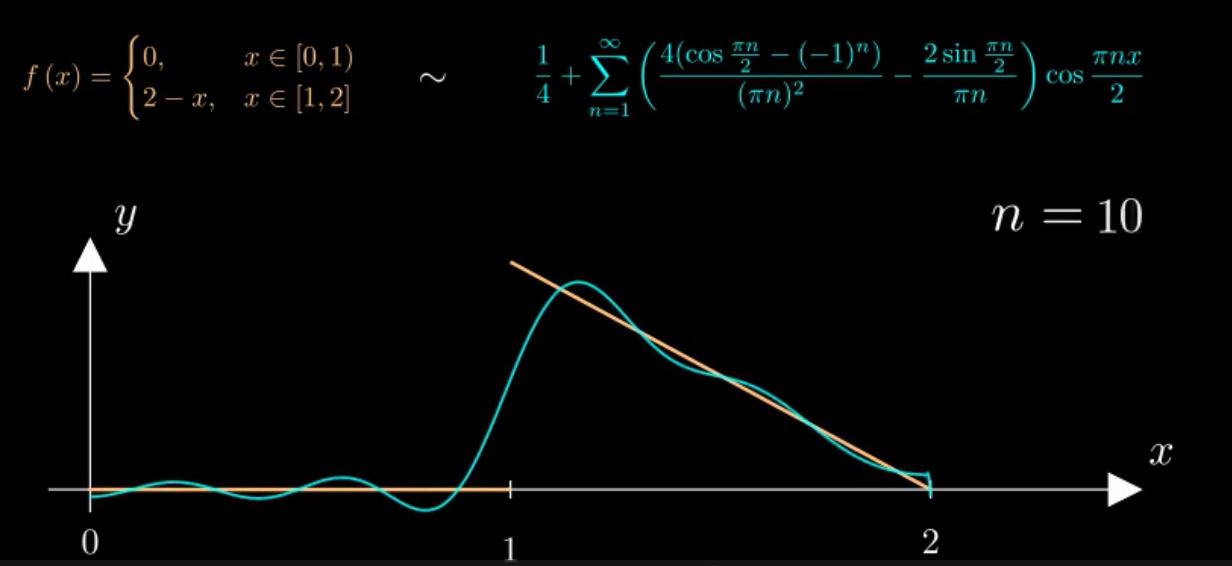
\includegraphics[width=\linewidth]{"./pictures/c_10.png"}
				\caption{при $n=10$}
			\end{subfigure}
			\begin{subfigure}{0.7\linewidth}
				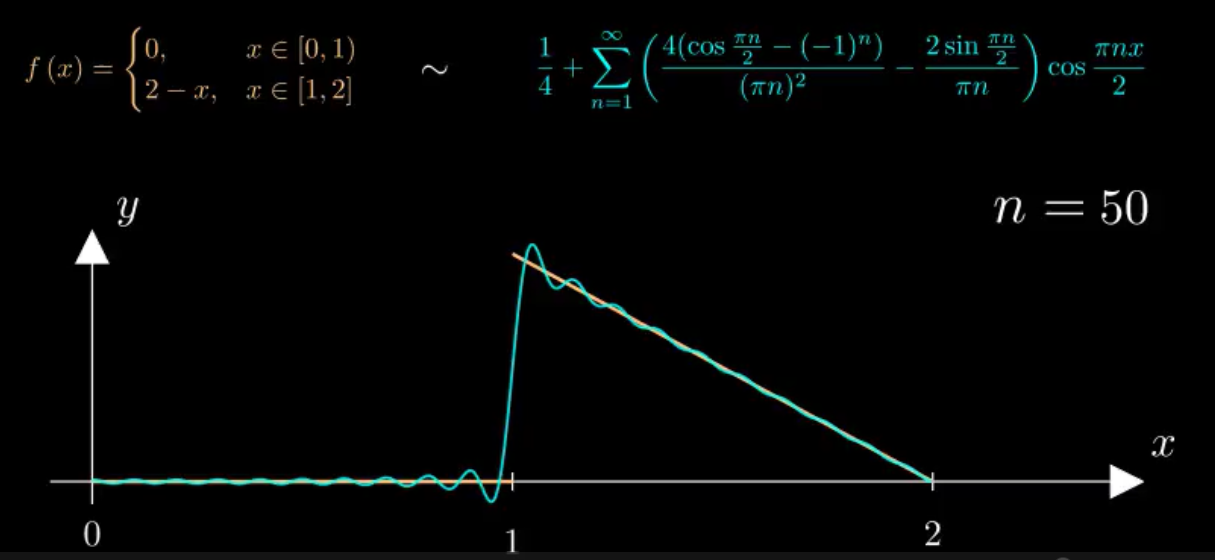
\includegraphics[width=\linewidth]{"./pictures/c_50.png"}
				\caption{при $n=50$}
			\end{subfigure}
		\caption{Результаты работы программы при различных $n$ для разложения в ряд Фурье по косинусам}\label{result}
		\end{center}
	\end{figure}

При увеличении $n$ заметно приближение исходной функции во всех трех случаях разложения в ряд Фурье. Образующиеся при больших $n$ "выбросы"  около точки 1 обусловлены неравномерной сходимостью ряда Фурье в точках разрыва (Рис. 4).


\begin{figure}[h]
		\center{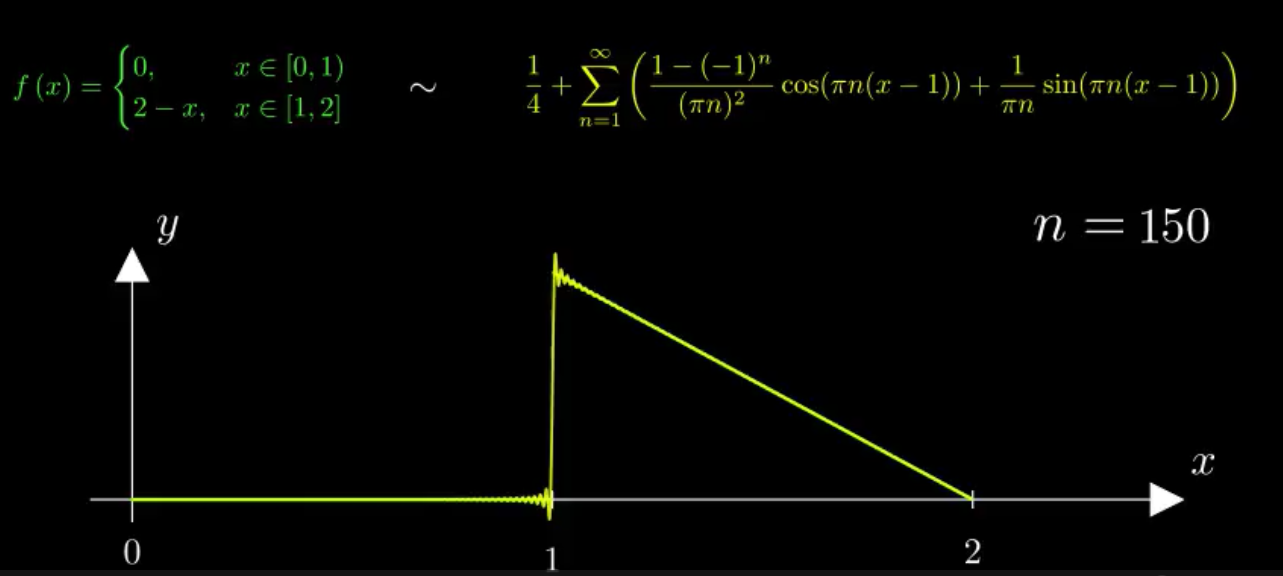
\includegraphics[width=1.0\linewidth]{"./pictures/max.png"}}
	           \caption{Результаты работы программы при $n = 150$ для общего тригонометрического ряда Фурье}
		
\label{ris:5}
\end{figure}


\newpage

\section{Нахождение суммы для каждого разложения в ряд Фурье}


\end{document}













